\documentclass{standalone}
\usepackage{tikz}
\usetikzlibrary{patterns, positioning}

\begin{document}
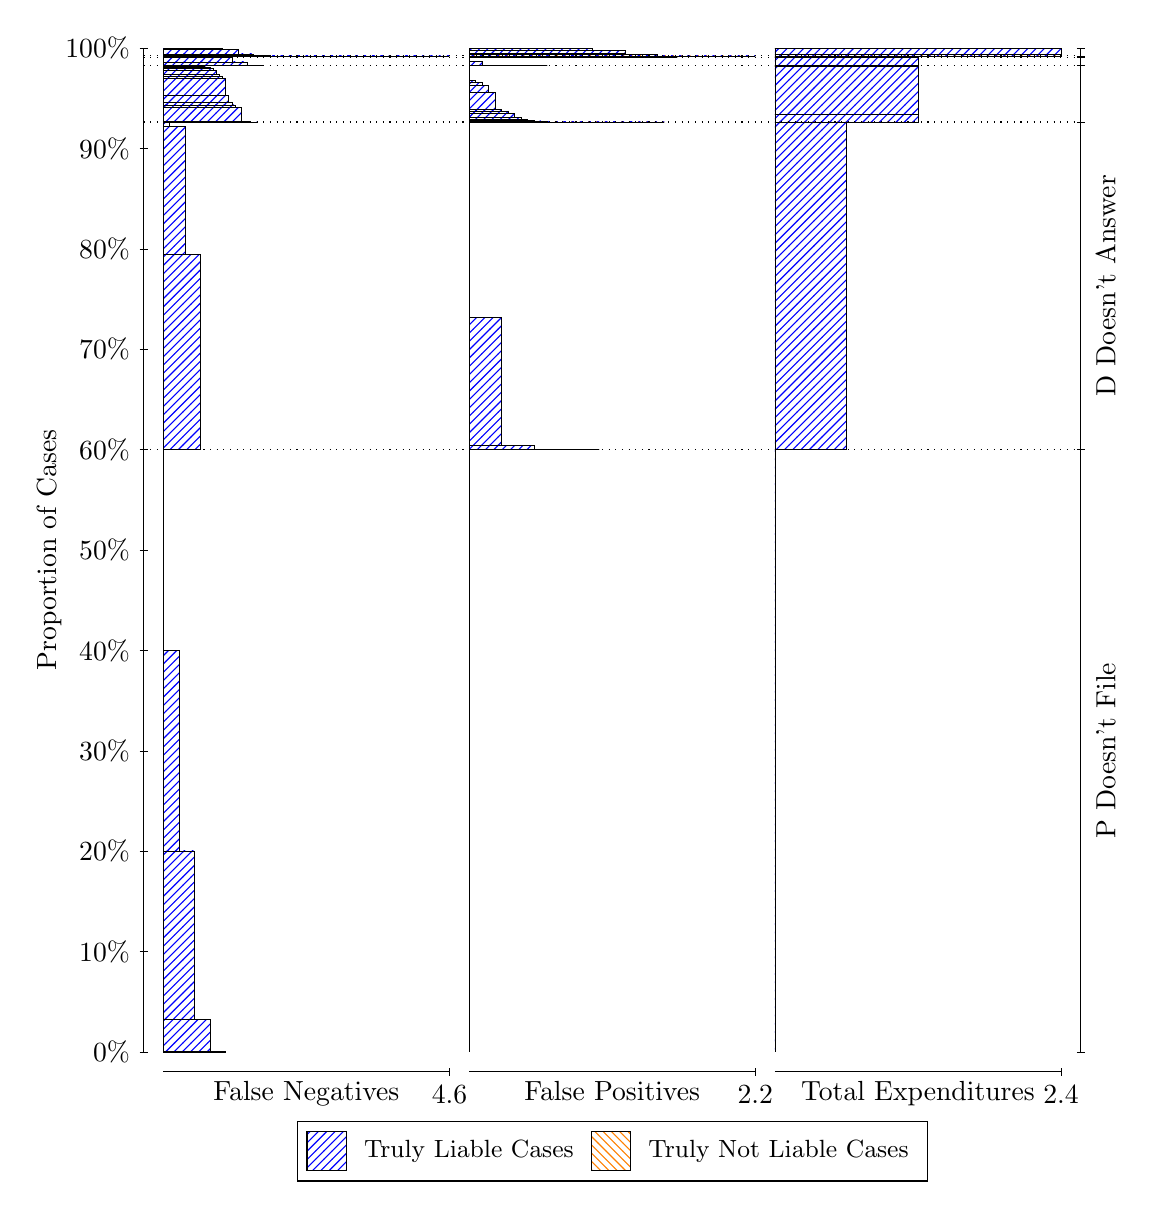
\begin{tikzpicture}
\draw[black, very thin] (1.5,1.75) -- (1.5,14.5);
\node[rotate=90, anchor=center] at (0.3, 8.125) {Proportion of Cases};
\draw[black, very thin] (1.45,1.75) -- (1.55,1.75);
\node[anchor=east] at (1.45, 1.75) {0\%};
\draw[black, very thin] (1.45,3.025) -- (1.55,3.025);
\node[anchor=east] at (1.45, 3.025) {10\%};
\draw[black, very thin] (1.45,4.3) -- (1.55,4.3);
\node[anchor=east] at (1.45, 4.3) {20\%};
\draw[black, very thin] (1.45,5.575) -- (1.55,5.575);
\node[anchor=east] at (1.45, 5.575) {30\%};
\draw[black, very thin] (1.45,6.85) -- (1.55,6.85);
\node[anchor=east] at (1.45, 6.85) {40\%};
\draw[black, very thin] (1.45,8.125) -- (1.55,8.125);
\node[anchor=east] at (1.45, 8.125) {50\%};
\draw[black, very thin] (1.45,9.4) -- (1.55,9.4);
\node[anchor=east] at (1.45, 9.4) {60\%};
\draw[black, very thin] (1.45,10.675) -- (1.55,10.675);
\node[anchor=east] at (1.45, 10.675) {70\%};
\draw[black, very thin] (1.45,11.95) -- (1.55,11.95);
\node[anchor=east] at (1.45, 11.95) {80\%};
\draw[black, very thin] (1.45,13.225) -- (1.55,13.225);
\node[anchor=east] at (1.45, 13.225) {90\%};
\draw[black, very thin] (1.45,14.5) -- (1.55,14.5);
\node[anchor=east] at (1.45, 14.5) {100\%};

\draw[black, very thin] (13.4,1.75) -- (13.4,14.5);
\draw[black, very thin] (13.35,1.75) -- (13.45,1.75);
\node[anchor=west] at (13.35, 1.75) {};
\draw[black, very thin] (13.35,9.4013) -- (13.45,9.4013);
\node[anchor=west] at (13.35, 9.4013) {};
\draw[black, very thin] (13.35,13.561) -- (13.45,13.561);
\node[anchor=west] at (13.35, 13.561) {};
\draw[black, very thin] (13.35,14.276) -- (13.45,14.276);
\node[anchor=west] at (13.35, 14.276) {};
\draw[black, very thin] (13.35,14.379) -- (13.45,14.379);
\node[anchor=west] at (13.35, 14.379) {};
\draw[black, very thin] (13.35,14.4) -- (13.45,14.4);
\node[anchor=west] at (13.35, 14.4) {};
\draw[black, very thin] (13.35,14.5) -- (13.45,14.5);
\node[anchor=west] at (13.35, 14.5) {};

\draw[black, very thin, pattern color=blue, pattern=north east lines] (1.75,1.75) rectangle (2.5399,1.7541);
\draw[black, very thin, pattern color=blue, pattern=north east lines] (1.75,1.7541) rectangle (2.3424,2.1592);
\draw[black, very thin, pattern color=blue, pattern=north east lines] (1.75,2.1592) rectangle (2.1449,4.3047);
\draw[black, very thin, pattern color=blue, pattern=north east lines] (1.75,4.3047) rectangle (1.9475,6.8513);
\draw[black, very thin, pattern color=orange, pattern=north west lines] (1.75,6.8513) rectangle (1.75,6.8513);
\draw[black, very thin, pattern color=blue, pattern=north east lines] (1.75,6.8513) rectangle (1.75,9.4013);
\draw[black, very thin, pattern color=blue, pattern=north east lines] (1.75,9.4013) rectangle (2.2239,11.884);
\draw[black, very thin, pattern color=blue, pattern=north east lines] (1.75,11.884) rectangle (2.0264,13.505);
\draw[black, very thin, pattern color=blue, pattern=north east lines] (1.75,13.505) rectangle (1.829,13.561);
\draw[black, very thin, pattern color=orange, pattern=north west lines] (1.75,13.561) rectangle (1.75,13.561);
\draw[black, very thin, pattern color=blue, pattern=north east lines] (1.75,13.561) rectangle (1.75,13.561);
\draw[black, very thin, pattern color=blue, pattern=north east lines] (1.75,13.561) rectangle (2.9348,13.563);
\draw[black, very thin, pattern color=blue, pattern=north east lines] (1.75,13.563) rectangle (2.8558,13.564);
\draw[black, very thin, pattern color=blue, pattern=north east lines] (1.75,13.564) rectangle (2.7768,13.569);
\draw[black, very thin, pattern color=blue, pattern=north east lines] (1.75,13.569) rectangle (2.7373,13.743);
\draw[black, very thin, pattern color=blue, pattern=north east lines] (1.75,13.743) rectangle (2.6978,13.744);
\draw[black, very thin, pattern color=blue, pattern=north east lines] (1.75,13.744) rectangle (2.6583,13.778);
\draw[black, very thin, pattern color=blue, pattern=north east lines] (1.75,13.778) rectangle (2.6188,13.809);
\draw[black, very thin, pattern color=blue, pattern=north east lines] (1.75,13.809) rectangle (2.5793,13.9);
\draw[black, very thin, pattern color=blue, pattern=north east lines] (1.75,13.9) rectangle (2.5399,14.113);
\draw[black, very thin, pattern color=blue, pattern=north east lines] (1.75,14.113) rectangle (2.5004,14.136);
\draw[black, very thin, pattern color=blue, pattern=north east lines] (1.75,14.136) rectangle (2.4609,14.141);
\draw[black, very thin, pattern color=blue, pattern=north east lines] (1.75,14.141) rectangle (2.4609,14.163);
\draw[black, very thin, pattern color=blue, pattern=north east lines] (1.75,14.163) rectangle (2.4214,14.22);
\draw[black, very thin, pattern color=blue, pattern=north east lines] (1.75,14.22) rectangle (2.3819,14.246);
\draw[black, very thin, pattern color=blue, pattern=north east lines] (1.75,14.246) rectangle (2.3819,14.246);
\draw[black, very thin, pattern color=blue, pattern=north east lines] (1.75,14.246) rectangle (2.3424,14.256);
\draw[black, very thin, pattern color=blue, pattern=north east lines] (1.75,14.256) rectangle (2.3029,14.261);
\draw[black, very thin, pattern color=blue, pattern=north east lines] (1.75,14.261) rectangle (2.2634,14.267);
\draw[black, very thin, pattern color=blue, pattern=north east lines] (1.75,14.267) rectangle (2.2634,14.267);
\draw[black, very thin, pattern color=blue, pattern=north east lines] (1.75,14.267) rectangle (2.2239,14.274);
\draw[black, very thin, pattern color=blue, pattern=north east lines] (1.75,14.274) rectangle (2.1844,14.275);
\draw[black, very thin, pattern color=blue, pattern=north east lines] (1.75,14.275) rectangle (2.1844,14.275);
\draw[black, very thin, pattern color=blue, pattern=north east lines] (1.75,14.275) rectangle (2.1449,14.275);
\draw[black, very thin, pattern color=blue, pattern=north east lines] (1.75,14.275) rectangle (2.1054,14.275);
\draw[black, very thin, pattern color=blue, pattern=north east lines] (1.75,14.275) rectangle (2.1054,14.275);
\draw[black, very thin, pattern color=blue, pattern=north east lines] (1.75,14.275) rectangle (2.0659,14.276);
\draw[black, very thin, pattern color=blue, pattern=north east lines] (1.75,14.276) rectangle (2.0659,14.276);
\draw[black, very thin, pattern color=blue, pattern=north east lines] (1.75,14.276) rectangle (2.0264,14.276);
\draw[black, very thin, pattern color=blue, pattern=north east lines] (1.75,14.276) rectangle (1.987,14.276);
\draw[black, very thin, pattern color=blue, pattern=north east lines] (1.75,14.276) rectangle (1.987,14.276);
\draw[black, very thin, pattern color=blue, pattern=north east lines] (1.75,14.276) rectangle (1.9475,14.276);
\draw[black, very thin, pattern color=blue, pattern=north east lines] (1.75,14.276) rectangle (1.908,14.276);
\draw[black, very thin, pattern color=blue, pattern=north east lines] (1.75,14.276) rectangle (1.908,14.276);
\draw[black, very thin, pattern color=blue, pattern=north east lines] (1.75,14.276) rectangle (1.8685,14.276);
\draw[black, very thin, pattern color=blue, pattern=north east lines] (1.75,14.276) rectangle (1.829,14.276);
\draw[black, very thin, pattern color=blue, pattern=north east lines] (1.75,14.276) rectangle (1.7895,14.276);
\draw[black, very thin, pattern color=orange, pattern=north west lines] (1.75,14.276) rectangle (1.75,14.276);
\draw[black, very thin, pattern color=blue, pattern=north east lines] (1.75,14.276) rectangle (1.75,14.276);
\draw[black, very thin, pattern color=blue, pattern=north east lines] (1.75,14.276) rectangle (3.0138,14.276);
\draw[black, very thin, pattern color=blue, pattern=north east lines] (1.75,14.276) rectangle (2.8163,14.323);
\draw[black, very thin, pattern color=blue, pattern=north east lines] (1.75,14.323) rectangle (2.6188,14.379);
\draw[black, very thin, pattern color=blue, pattern=north east lines] (1.75,14.379) rectangle (2.4214,14.379);
\draw[black, very thin, pattern color=blue, pattern=north east lines] (1.75,14.379) rectangle (2.2239,14.379);
\draw[black, very thin, pattern color=orange, pattern=north west lines] (1.75,14.379) rectangle (1.75,14.379);
\draw[black, very thin, pattern color=blue, pattern=north east lines] (1.75,14.379) rectangle (2.2239,14.386);
\draw[black, very thin, pattern color=blue, pattern=north east lines] (1.75,14.386) rectangle (2.0264,14.398);
\draw[black, very thin, pattern color=blue, pattern=north east lines] (1.75,14.398) rectangle (1.829,14.4);
\draw[black, very thin, pattern color=orange, pattern=north west lines] (1.75,14.4) rectangle (1.75,14.4);
\draw[black, very thin, pattern color=blue, pattern=north east lines] (1.75,14.4) rectangle (1.75,14.4);
\draw[black, very thin, pattern color=blue, pattern=north east lines] (1.75,14.4) rectangle (5.3833,14.4);
\draw[black, very thin, pattern color=blue, pattern=north east lines] (1.75,14.4) rectangle (5.1859,14.4);
\draw[black, very thin, pattern color=blue, pattern=north east lines] (1.75,14.4) rectangle (4.9884,14.401);
\draw[black, very thin, pattern color=blue, pattern=north east lines] (1.75,14.401) rectangle (4.7909,14.401);
\draw[black, very thin, pattern color=blue, pattern=north east lines] (1.75,14.401) rectangle (4.5935,14.401);
\draw[black, very thin, pattern color=blue, pattern=north east lines] (1.75,14.401) rectangle (4.396,14.401);
\draw[black, very thin, pattern color=blue, pattern=north east lines] (1.75,14.401) rectangle (4.1986,14.401);
\draw[black, very thin, pattern color=blue, pattern=north east lines] (1.75,14.401) rectangle (3.2902,14.401);
\draw[black, very thin, pattern color=blue, pattern=north east lines] (1.75,14.401) rectangle (3.0928,14.403);
\draw[black, very thin, pattern color=blue, pattern=north east lines] (1.75,14.403) rectangle (2.8953,14.426);
\draw[black, very thin, pattern color=blue, pattern=north east lines] (1.75,14.426) rectangle (2.6978,14.478);
\draw[black, very thin, pattern color=blue, pattern=north east lines] (1.75,14.478) rectangle (2.5004,14.5);
\draw[black, very thin, pattern color=blue, pattern=north east lines] (1.75,14.5) rectangle (2.3029,14.5);
\draw[black, very thin, pattern color=blue, pattern=north east lines] (1.75,14.5) rectangle (2.1054,14.5);
\draw[black, very thin, pattern color=blue, pattern=north east lines] (1.75,14.5) rectangle (1.908,14.5);
\draw[black, very thin, pattern color=orange, pattern=north west lines] (1.75,14.5) rectangle (1.75,14.5);
\draw[black, very thin, pattern color=orange, pattern=north west lines] (5.6333,1.75) rectangle (5.6333,1.75);
\draw[black, very thin, pattern color=blue, pattern=north east lines] (5.6333,1.75) rectangle (5.6333,9.4013);
\draw[black, very thin, pattern color=orange, pattern=north west lines] (5.6333,9.4013) rectangle (7.2848,9.4013);
\draw[black, very thin, pattern color=blue, pattern=north east lines] (5.6333,9.4013) rectangle (7.2848,9.4013);
\draw[black, very thin, pattern color=blue, pattern=north east lines] (5.6333,9.4013) rectangle (6.872,9.4013);
\draw[black, very thin, pattern color=blue, pattern=north east lines] (5.6333,9.4013) rectangle (6.4591,9.4575);
\draw[black, very thin, pattern color=blue, pattern=north east lines] (5.6333,9.4575) rectangle (6.0462,11.079);
\draw[black, very thin, pattern color=blue, pattern=north east lines] (5.6333,11.079) rectangle (5.6333,13.561);
\draw[black, very thin, pattern color=orange, pattern=north west lines] (5.6333,13.561) rectangle (8.1106,13.561);
\draw[black, very thin, pattern color=blue, pattern=north east lines] (5.6333,13.561) rectangle (8.1106,13.561);
\draw[black, very thin, pattern color=orange, pattern=north west lines] (5.6333,13.561) rectangle (7.9455,13.561);
\draw[black, very thin, pattern color=blue, pattern=north east lines] (5.6333,13.561) rectangle (7.9455,13.561);
\draw[black, very thin, pattern color=orange, pattern=north west lines] (5.6333,13.561) rectangle (7.7803,13.561);
\draw[black, very thin, pattern color=blue, pattern=north east lines] (5.6333,13.561) rectangle (7.7803,13.561);
\draw[black, very thin, pattern color=blue, pattern=north east lines] (5.6333,13.561) rectangle (7.6977,13.561);
\draw[black, very thin, pattern color=orange, pattern=north west lines] (5.6333,13.561) rectangle (7.6152,13.561);
\draw[black, very thin, pattern color=blue, pattern=north east lines] (5.6333,13.561) rectangle (7.6152,13.561);
\draw[black, very thin, pattern color=blue, pattern=north east lines] (5.6333,13.561) rectangle (7.5326,13.561);
\draw[black, very thin, pattern color=orange, pattern=north west lines] (5.6333,13.561) rectangle (7.45,13.561);
\draw[black, very thin, pattern color=blue, pattern=north east lines] (5.6333,13.561) rectangle (7.45,13.561);
\draw[black, very thin, pattern color=blue, pattern=north east lines] (5.6333,13.561) rectangle (7.3674,13.561);
\draw[black, very thin, pattern color=orange, pattern=north west lines] (5.6333,13.561) rectangle (7.2848,13.561);
\draw[black, very thin, pattern color=blue, pattern=north east lines] (5.6333,13.561) rectangle (7.2848,13.561);
\draw[black, very thin, pattern color=blue, pattern=north east lines] (5.6333,13.561) rectangle (7.2023,13.561);
\draw[black, very thin, pattern color=orange, pattern=north west lines] (5.6333,13.561) rectangle (7.1197,13.561);
\draw[black, very thin, pattern color=blue, pattern=north east lines] (5.6333,13.561) rectangle (7.1197,13.561);
\draw[black, very thin, pattern color=blue, pattern=north east lines] (5.6333,13.561) rectangle (7.0371,13.561);
\draw[black, very thin, pattern color=orange, pattern=north west lines] (5.6333,13.561) rectangle (6.9545,13.561);
\draw[black, very thin, pattern color=blue, pattern=north east lines] (5.6333,13.561) rectangle (6.9545,13.561);
\draw[black, very thin, pattern color=blue, pattern=north east lines] (5.6333,13.561) rectangle (6.9545,13.562);
\draw[black, very thin, pattern color=blue, pattern=north east lines] (5.6333,13.562) rectangle (6.872,13.562);
\draw[black, very thin, pattern color=orange, pattern=north west lines] (5.6333,13.562) rectangle (6.7894,13.562);
\draw[black, very thin, pattern color=blue, pattern=north east lines] (5.6333,13.562) rectangle (6.7894,13.563);
\draw[black, very thin, pattern color=blue, pattern=north east lines] (5.6333,13.563) rectangle (6.7068,13.563);
\draw[black, very thin, pattern color=blue, pattern=north east lines] (5.6333,13.563) rectangle (6.6242,13.57);
\draw[black, very thin, pattern color=blue, pattern=north east lines] (5.6333,13.57) rectangle (6.5417,13.57);
\draw[black, very thin, pattern color=blue, pattern=north east lines] (5.6333,13.57) rectangle (6.5417,13.576);
\draw[black, very thin, pattern color=blue, pattern=north east lines] (5.6333,13.576) rectangle (6.4591,13.581);
\draw[black, very thin, pattern color=blue, pattern=north east lines] (5.6333,13.581) rectangle (6.3765,13.591);
\draw[black, very thin, pattern color=blue, pattern=north east lines] (5.6333,13.591) rectangle (6.2939,13.617);
\draw[black, very thin, pattern color=blue, pattern=north east lines] (5.6333,13.617) rectangle (6.2114,13.674);
\draw[black, very thin, pattern color=blue, pattern=north east lines] (5.6333,13.674) rectangle (6.1288,13.696);
\draw[black, very thin, pattern color=blue, pattern=north east lines] (5.6333,13.696) rectangle (6.1288,13.701);
\draw[black, very thin, pattern color=blue, pattern=north east lines] (5.6333,13.701) rectangle (6.0462,13.724);
\draw[black, very thin, pattern color=blue, pattern=north east lines] (5.6333,13.724) rectangle (5.9636,13.937);
\draw[black, very thin, pattern color=blue, pattern=north east lines] (5.6333,13.937) rectangle (5.8811,14.028);
\draw[black, very thin, pattern color=blue, pattern=north east lines] (5.6333,14.028) rectangle (5.7985,14.059);
\draw[black, very thin, pattern color=blue, pattern=north east lines] (5.6333,14.059) rectangle (5.7159,14.093);
\draw[black, very thin, pattern color=blue, pattern=north east lines] (5.6333,14.093) rectangle (5.6333,14.276);
\draw[black, very thin, pattern color=orange, pattern=north west lines] (5.6333,14.276) rectangle (6.6242,14.276);
\draw[black, very thin, pattern color=blue, pattern=north east lines] (5.6333,14.276) rectangle (6.6242,14.276);
\draw[black, very thin, pattern color=blue, pattern=north east lines] (5.6333,14.276) rectangle (6.2114,14.276);
\draw[black, very thin, pattern color=blue, pattern=north east lines] (5.6333,14.276) rectangle (5.7985,14.332);
\draw[black, very thin, pattern color=blue, pattern=north east lines] (5.6333,14.332) rectangle (5.6333,14.379);
\draw[black, very thin, pattern color=orange, pattern=north west lines] (5.6333,14.379) rectangle (8.2758,14.379);
\draw[black, very thin, pattern color=blue, pattern=north east lines] (5.6333,14.379) rectangle (8.2758,14.379);
\draw[black, very thin, pattern color=blue, pattern=north east lines] (5.6333,14.379) rectangle (7.8629,14.379);
\draw[black, very thin, pattern color=blue, pattern=north east lines] (5.6333,14.379) rectangle (7.45,14.381);
\draw[black, very thin, pattern color=blue, pattern=north east lines] (5.6333,14.381) rectangle (7.0371,14.393);
\draw[black, very thin, pattern color=blue, pattern=north east lines] (5.6333,14.393) rectangle (6.6242,14.4);
\draw[black, very thin, pattern color=orange, pattern=north west lines] (5.6333,14.4) rectangle (9.2667,14.4);
\draw[black, very thin, pattern color=blue, pattern=north east lines] (5.6333,14.4) rectangle (9.2667,14.4);
\draw[black, very thin, pattern color=blue, pattern=north east lines] (5.6333,14.4) rectangle (8.8538,14.4);
\draw[black, very thin, pattern color=orange, pattern=north west lines] (5.6333,14.4) rectangle (8.8538,14.4);
\draw[black, very thin, pattern color=blue, pattern=north east lines] (5.6333,14.4) rectangle (8.8538,14.4);
\draw[black, very thin, pattern color=blue, pattern=north east lines] (5.6333,14.4) rectangle (8.4409,14.401);
\draw[black, very thin, pattern color=orange, pattern=north west lines] (5.6333,14.401) rectangle (8.4409,14.401);
\draw[black, very thin, pattern color=blue, pattern=north east lines] (5.6333,14.401) rectangle (8.4409,14.401);
\draw[black, very thin, pattern color=blue, pattern=north east lines] (5.6333,14.401) rectangle (8.028,14.418);
\draw[black, very thin, pattern color=orange, pattern=north west lines] (5.6333,14.418) rectangle (8.028,14.418);
\draw[black, very thin, pattern color=blue, pattern=north east lines] (5.6333,14.418) rectangle (8.028,14.422);
\draw[black, very thin, pattern color=blue, pattern=north east lines] (5.6333,14.422) rectangle (7.6152,14.427);
\draw[black, very thin, pattern color=blue, pattern=north east lines] (5.6333,14.427) rectangle (7.6152,14.474);
\draw[black, very thin, pattern color=blue, pattern=north east lines] (5.6333,14.474) rectangle (7.2023,14.497);
\draw[black, very thin, pattern color=blue, pattern=north east lines] (5.6333,14.497) rectangle (6.7894,14.499);
\draw[black, very thin, pattern color=blue, pattern=north east lines] (5.6333,14.499) rectangle (6.3765,14.499);
\draw[black, very thin, pattern color=orange, pattern=north west lines] (5.6333,14.499) rectangle (5.6333,14.499);
\draw[black, very thin, pattern color=blue, pattern=north east lines] (5.6333,14.499) rectangle (5.6333,14.5);
\draw[black, very thin, pattern color=orange, pattern=north west lines] (9.5167,1.75) rectangle (9.5167,1.75);
\draw[black, very thin, pattern color=blue, pattern=north east lines] (9.5167,1.75) rectangle (9.5167,9.4013);
\draw[black, very thin, pattern color=orange, pattern=north west lines] (9.5167,9.4013) rectangle (10.425,9.4013);
\draw[black, very thin, pattern color=blue, pattern=north east lines] (9.5167,9.4013) rectangle (10.425,13.561);
\draw[black, very thin, pattern color=orange, pattern=north west lines] (9.5167,13.561) rectangle (11.333,13.561);
\draw[black, very thin, pattern color=blue, pattern=north east lines] (9.5167,13.561) rectangle (11.333,13.656);
\draw[black, very thin, pattern color=orange, pattern=north west lines] (9.5167,13.656) rectangle (11.333,13.656);
\draw[black, very thin, pattern color=blue, pattern=north east lines] (9.5167,13.656) rectangle (11.333,14.264);
\draw[black, very thin, pattern color=orange, pattern=north west lines] (9.5167,14.264) rectangle (11.333,14.264);
\draw[black, very thin, pattern color=blue, pattern=north east lines] (9.5167,14.264) rectangle (11.333,14.276);
\draw[black, very thin, pattern color=orange, pattern=north west lines] (9.5167,14.276) rectangle (11.333,14.276);
\draw[black, very thin, pattern color=blue, pattern=north east lines] (9.5167,14.276) rectangle (11.333,14.379);
\draw[black, very thin, pattern color=orange, pattern=north west lines] (9.5167,14.379) rectangle (11.333,14.379);
\draw[black, very thin, pattern color=blue, pattern=north east lines] (9.5167,14.379) rectangle (11.333,14.4);
\draw[black, very thin, pattern color=orange, pattern=north west lines] (9.5167,14.4) rectangle (13.15,14.4);
\draw[black, very thin, pattern color=blue, pattern=north east lines] (9.5167,14.4) rectangle (13.15,14.422);
\draw[black, very thin, pattern color=orange, pattern=north west lines] (9.5167,14.422) rectangle (13.15,14.422);
\draw[black, very thin, pattern color=blue, pattern=north east lines] (9.5167,14.422) rectangle (13.15,14.499);
\draw[black, very thin, pattern color=orange, pattern=north west lines] (9.5167,14.499) rectangle (13.15,14.499);
\draw[black, very thin, pattern color=blue, pattern=north east lines] (9.5167,14.499) rectangle (13.15,14.5);
\draw[black, dotted] (1.5,9.4013) -- (13.4,9.4013);
\draw[black, dotted] (1.5,13.561) -- (13.4,13.561);
\draw[black, dotted] (1.5,14.276) -- (13.4,14.276);
\draw[black, dotted] (1.5,14.379) -- (13.4,14.379);
\draw[black, dotted] (1.5,14.4) -- (13.4,14.4);
\draw[black, very thin] (1.75,1.5) -- (5.3833,1.5);
\node[anchor=north] at (3.5667, 1.5) {False Negatives};
\draw[black, very thin] (5.3833,1.45) -- (5.3833,1.55);
\node[anchor=north] at (5.3833, 1.45) {4.6};

\draw[black, very thin] (5.6333,1.5) -- (9.2667,1.5);
\node[anchor=north] at (7.45, 1.5) {False Positives};
\draw[black, very thin] (9.2667,1.45) -- (9.2667,1.55);
\node[anchor=north] at (9.2667, 1.45) {2.2};

\draw[black, very thin] (9.5167,1.5) -- (13.15,1.5);
\node[anchor=north] at (11.333, 1.5) {Total Expenditures};
\draw[black, very thin] (13.15,1.45) -- (13.15,1.55);
\node[anchor=north] at (13.15, 1.45) {2.4};

\node[black, centered, rotate=90] at (13.72, 5.5756) {P Doesn't File};
\node[black, centered, rotate=90] at (13.72, 11.481) {D Doesn't Answer};





\draw (7.449999999999999,1.5) node[draw=none] (baseCoordinate) {};
\begin{scope}[align=center]
        \matrix[scale=0.5, draw=black, below=0.5cm of baseCoordinate, nodes={draw}, column sep=0.1cm]{
            \node[rectangle, draw, minimum width=0.5cm, minimum height=0.5cm, pattern=north east lines, pattern color=blue] {}; &
            \node[draw=none, font=\small] (B) {Truly Liable Cases}; &
            \node[rectangle, draw, minimum width=0.5cm, minimum height=0.5cm, pattern=north west lines, pattern color=orange] {}; &
            \node[draw=none, font=\small] (B) {Truly Not Liable Cases}; \\
            };
\end{scope}

\end{tikzpicture}
\end{document}